\documentclass{standalone}
%<--------------------------------------------------------------------------->%
%%% TikZ %%%
\usepackage{tikz}
% \usetikzlibrary{calc}
% \usetikzlibrary{angles,quotes}
% \usetikzlibrary{intersections,topaths}
% \usetikzlibrary{decorations.markings}
%<--------------------------------------------------------------------------->%

\begin{document}

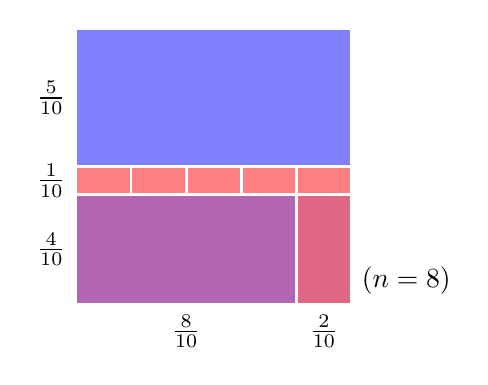
\begin{tikzpicture}[scale=3.5,thick,line cap=round]
	\tikzstyle{jiao}=[solid,circle,draw,fill=white,inner sep=.8pt];
	\tikzstyle{tile1}=[line width=0.1em,draw=white,fill=blue!50];
\tikzstyle{tile2}=[line width=0.1em,draw=white,fill=red!50];
\tikzstyle{tile3}=[line width=0.1em,draw=white,fill=blue!50!red!60];
\tikzstyle{tile4}=[line width=0.1em,draw=white,fill=blue!20!red!60];

	\draw[tile3] (0,0)     rectangle (4/5,2/5);
	\draw[tile4] (4/5,0)   rectangle (1,2/5);
	\draw[tile1] (0,1)     rectangle (1,1/2);
	\draw[tile2] (0/5,2/5) rectangle +(1/5,1/10);
	\draw[tile2] (1/5,2/5) rectangle +(1/5,1/10);
	\draw[tile2] (2/5,2/5) rectangle +(1/5,1/10);
	\draw[tile2] (3/5,2/5) rectangle +(1/5,1/10);
	\draw[tile2] (4/5,2/5) rectangle +(1/5,1/10);
	\node[left]  at (0,1/5)    {$\frac4{10}$};
	\node[left]  at (0,4.5/10) {$\frac1{10}$};
	\node[left]  at (0,3/4)    {$\frac5{10}$};
	\node[below] at (2/5,0)    {$\frac8{10}$};
	\node[below] at (9/10,0)   {$\frac2{10}$};
	\node[above right] at (1,0) {$(n=8)$};
\end{tikzpicture}

\end{document}
